%! Author = kevin
%! Date = 31/08/2023

% Preamble
\documentclass{report}

% Packages
\usepackage{graphicx}
\usepackage{enumerate}
\usepackage[spanish,es-tabla]{babel}
\usepackage[utf8]{inputenc}
\usepackage{amsmath,amssymb}
\usepackage[usenames]{color}
\usepackage[dvipsnames]{xcolor}
\usepackage[T1]{fontenc}
\usepackage{listings}
\usepackage[hidelinks]{hyperref}
\usepackage{subfiles}

%habilitar colorear enlaces
\hypersetup{ colorlinks=true,
             linkcolor=black,
             filecolor=magenta,
             urlcolor=cyan,
            }

\definecolor{codegreen}{rgb}{0,0.6,0}
\definecolor{codegray}{rgb}{0.5,0.5,0.5}
\definecolor{codepurple}{HTML}{C42043}
\definecolor{backcolour}{HTML}{F2F2F2}
\definecolor{bookColor}{cmyk}{0,0,0,0.90}
\color{bookColor}

\lstset{upquote=true}

\lstdefinestyle{customPython}{
  language=Python,
  basicstyle=\small\ttfamily,
  keywordstyle=\color{blue},
  commentstyle=\color{green!40!black},
  stringstyle=\color{purple},
  numbers=left,
  numberstyle=\tiny\color{gray},
  stepnumber=1,
  tabsize=4,
  showspaces=false,
  showstringspaces=false
}

\lstset{style=customPython}

\newcommand\numberstyle[1]{%
    \footnotesize
    \color{codegray}%
    \ttfamily
    \ifnum#1<10 0\fi#1 |%
}

% Document
\begin{document}

\begin{titlepage}
    \centering
    {\scshape\Huge Linear Regression\par}
    \vspace{0.5cm}
    {\itshape\Large Laboratirio N°1 - Introduccion a Machine Learning \par}
    \vspace{0.5cm}
    {\Large Agosto 2023 \par}
    \vspace{0.5cm}
    {
\includegraphics[width=0.5\textwidth]{latex/utec.jpg}\par}
    \vfill
    {\Large Integrantes: \par}
    {\Large Juan Diego Castro Padilla\par}
    {\Large Kevin Abraham Huaman Vega\par}
    {\Large Juan Diego Prochazka Zegarra\par}
    \vfill
    %(100\%)
    \vspace{0.5cm}
    {\bfseries\LARGE Universidad de Ingenier\'ia y Tecnolog\'ia\par}
    \vspace{0.5cm}
    {\scshape\Large Facultad de Computaci\'on \par}
    \vspace{0.5cm}
    {\Large Docente: Arturo Deza\par}
    \vspace{0.5cm}
    {\Large 2023-2 \par}
    \vspace{1.5cm}

\end{titlepage}

\tableofcontents

\pagebreak

\noindent

    \chapter{Desarrollo}
        \section{What is your dataset ?}
            Nuestro dataset fue extra\'ido de \href{https://www.kaggle.com}{kaggle.com}. El nombre del dataset es \textbf{Most Streamed Spotify Songs 2023}, y tiene como alcance principal proporcionar informaci\'on sobre la plataforma que permitan encontrar insights entre los usuarios y el \'exito que llegan a alcanzar algunas canciones. El conjunto de atributos disponibles en el dataset son referentes al nombre de la canci\'on, el/los cantantes, fecha de lanzamiento, cantidad de reproducciones, cantidad de usuarios que han incluido la cancion en su playlist, entre otros.
            La referencia al dataset se encuentra en el cap\'itulo 4.

        \section{What is your regression problem?}
            Queremos determinar si existe una relaci\'on fuerte entre la cantidad de reproducciones de una canci\'on con la cantidad de usuarios que pusieron dicha canci\'on en su playlist, con la intenci\'on de predecir la cantidad de usuarios que pondr\'an una canci\'on en su playlist dado un n\'umero de reproducciones. Nuestra hip\'otesis preliminar sugiere que mientras mas reproducciones tenga una canci\'on de en Spotify m\'as personas decidir\'an agregar dicha canci\'on en su playlist. Creemos que nuestra hip\'otesis tiene sentido l\'ogico puesto que generalmente los usuarios deciden poner una canci\'on en su playlist posterior a haberla escuchado (y que les haya agradado). Por lo tanto, si mas personas escuchan la canci\'on creemos que hay chance de que le guste a m\'as personas y la agreguen a su playlist.
        \section{How many data points are there in the dataset?}
            Para este laboratorio vamos a trabajar con un subconjunto del dataset original, puesto que estamos reduciendo el scope de nuestro estudio a canciones actuales. Vamos a trabajar en el rango de canciones del 2021 al 2022. Esta reducci\'on nos deja con 521 puntos para analizar.
        \section{What is the β term assuming a zero-th point intersection (no bias)}
            $ \[\beta\] = 0.7371 $
        \section{What is the bias term not assuming a zero\-th point intersection (bias included)}
            $ bias = 156.6146 $
        \section{What are the number of independent variables (minimum 1, maximum 2)}
            Estamos usando 1 variable independiente.

        \section{What is the dependent variable?}
            Nuestra variable dependiente es \textbf{in\_spotify\_playlists} que simboliza la cantidad de playlists donde una canci\'on est\'a incluida

        \section{What are the unit of measurements for each variable(s)?}
            La variable independiente \textbf{streams}, que simboliza la cantidad de reproducciones de una canci\'on de Spotify, se mide en cientos de miles de reproducciones. Por otra parte, la variable dependiente \textbf{in\_spotify\_playlists}, que es la cantidad de playlists donde la canci\'on esta incluida, se mide en unidades.

        \section{Please plot the raw data and a superimposing line on the data that passes through the origin. What is the mean square error (MSE)?}
            {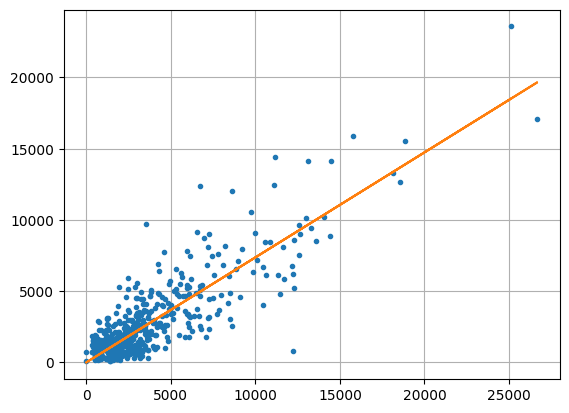
\includegraphics[width=0.9\textwidth]{latex/question9.png}\par} \\
            betha: 0.7370945213834329 \\
            mse: 2280789.90594258 playlists^2
        \section{Please plot the raw data and a superimposing line on the data that does not pass through the origin. What is the mean square error (MSE)?}
            {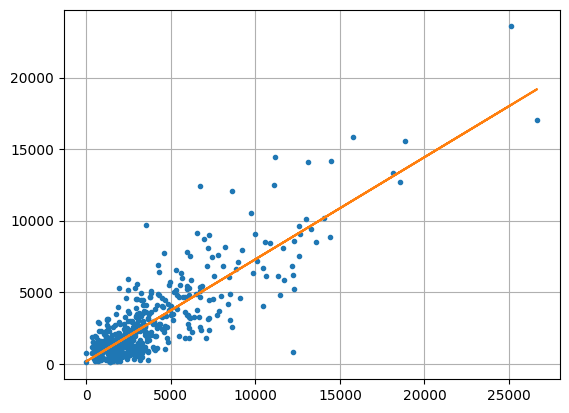
\includegraphics[width=0.9\textwidth]{latex/question10.png}\par} \\
            beta: 0.7141004053993129 \\
            bias: 156.61455673680575 \\
            mse: 0.721641373403032

        \section{ Statistical bootstrapping.}

        A continuaci\'on se encuentra el Bootstrapping, para el modelo lineal con y sin bias, en ese orden. La variable betaNoBias es el valor promedio del parametro de los modelos que pasan por cero. Las variables betaBias y biasBias son los valores promedio de los parametros beta y bias de los modelos que consideran un bias.

        \begin{lstlisting}
        # Bootstrapping
        # Linear no bias
        ITERS = 100

        betaNoBias = 0
        for i in range(0,ITERS):
            #avoid modifying all the datasets
            dataset_ = copy.deepcopy(dataset)
            dataset_.remove_obs(random.randint(0,
                    dataset_.n_elems() - 1))
            fit = LinearModel(dataset_)
            #calculate mean distributing the division
            betaNoBias += fit.get_beta()/ITERS


        betaBias = 0
        biasBias = 0
        for i in range(0,ITERS):
            #avoid modifying all the datasets
            dataset_ = copy.deepcopy(dataset)
            dataset_.remove_obs(random.randint(0, \
                dataset_.n_elems() - 1))
            fit = BiasLinearModel(dataset_)
            betaBias += fit.get_beta()/ITERS
            biasBias += fit.get_bias()/ITERS

        betaNoBias, (betaBias, biasBias)
        \end{lstlisting}

        output:
        (0.7368973293059682, (0.7139741003773192, 157.36196988749182))

\chapter{Contribuciones}
        \begin{itemize}
            \item Juan Diego Castro Padilla:

            Busqueda del dataset y creaci\'on de las clases Dataset y BiasLinearModel.
            \item Kevin Abraham Huaman Vega:

            An\'alisis y limpieza de la data para definir las variables a relacionar, investigación y redacci\'on del informe.

            \item Juan Diego Prochazka Zegarra:

            Creaci\'on de las clases LinearModel y StatisticalMeasures. Bootstrapping.

            \end{itemize}
\chapter{Paquetes}
    \begin{itemize}
        \item Matplotlib
        \item Pandas
        \item Numpy
        \item random
        \item copy
    \end{itemize}

\chapter{Lista de Herramientas}
    \subtitle{Dataset}
        \href{https://www.kaggle.com/datasets/nelgiriyewithana/top-spotify-songs-2023}{Most Streamed Spotify Songs 2023}.

    \subtitle{Licence}
        \href{https://opensource.org/license/mit/}{MIT license}
\chapter{C\'odigo fuente}
    \subtitle{Importar las librer\'ias}
    \begin{lstlisting}
    import matplotlib.pyplot as plt
    import pandas as pd
    import numpy as np
    import random
    import copy
    \end{lstlisting}

    \subtitle{Representaci\'on del dataset}
    \begin{lstlisting}
    class DataSet:
    x_var: str = None
    y_var: str = None
    x: np.array = None
    y: np.array = None

    def __init__(self, filename: str, x_variable_name: str,
        y_variable_name: str):

        _df = pd.read_csv(filename)

        self.x_var: str = x_variable_name
        self.y_var: str = y_variable_name

        self.x = np.array(_df[self.x_var])
        self.y = np.array(_df[self.y_var])

    def remove_obs(self, index):
        self.x = np.delete(self.x,index)
        self.y = np.delete(self.y,index)

    def n_elems(self):
        return self.x.size
    \end{lstlisting}

    \subtitle{Modelos}
    \begin{lstlisting}
    class LinearModel:
    dataset = None
    beta = None

    def _eval_point_with_params(self, x):
        return self.beta * x

    def _calculate_beta(self) -> float:
        numerator = np.sum(self.dataset.x * self.dataset.y)
        denominator = np.sum(np.power(self.dataset.x, 2))

        return numerator / denominator

    def __init__(self, _dataset):
        self.dataset = _dataset
        self.beta = self._calculate_beta()

    def predict(self, x):
        return self._eval_point_with_params(x)

    def get_beta(self):
        return self.beta

    def plot(self):
        y_hat = self.predict(self.dataset.x)

        plt.grid()
        plt.plot(self.dataset.x, self.dataset.y, '.')
        plt.plot(self.dataset.x, y_hat)
        plt.show()
    \end{lstlisting}

    \begin{lstlisting}
    class BiasLinearModel:
    dataset = None
    beta = None
    bias = None

    def _eval_point_with_params(self, x):
        return self.beta * x + self.bias

    def _calculate_beta(self) -> float:
        x_mean = np.mean(self.dataset.x)
        y_mean = np.mean(self.dataset.y)

        numerator = np.sum((self.dataset.x * self.dataset.y) \
            - (y_mean * self.dataset.x))
        denominator = np.sum(np.power(self.dataset.x, 2) \
            - x_mean * self.dataset.x)

        return numerator / denominator

    def _calculate_bias(self) -> float:
        x_mean = np.mean(self.dataset.x)
        y_mean = np.mean(self.dataset.y)

        return y_mean - self.get_beta() * x_mean

    def __init__(self, _dataset):
        self.dataset = _dataset
        self.beta = self._calculate_beta()
        self.bias = self._calculate_bias()

    def predict(self, x):
        return self._eval_point_with_params(x)

    def get_beta(self):
        return self.beta

    def get_bias(self):
        return self.bias

    def plot(self):
        y_hat = self.predict(self.dataset.x)

        plt.grid()
        plt.plot(self.dataset.x, self.dataset.y, '.')
        plt.plot(self.dataset.x, y_hat)
        plt.show()
    \end{lstlisting}

    \subtitle{Medidas estad\'isticas usadas para entender nuestra funci\'on de p\'erdida/errores:}
    \begin{lstlisting}
    class StatisticalMeasures:

    @staticmethod
    def mse(model: LinearModel | BiasLinearModel):
        y_hat = model.predict(model.dataset.x)

        terms = np.power(y_hat - model.dataset.y, 2)
        accm = np.sum(terms) / dataset.n_elems()
        return accm

    @staticmethod
    def r_squeared(model: LinearModel | BiasLinearModel):
        y_mean = np.mean(model.dataset.y)
        y_hat = model.predict(model.dataset.x)

        numerator = np.sum(np.power(model.dataset.y - y_hat, 2))
        denominator = np.sum(np.power(model.dataset.y - y_mean, 2))
        return 1 - numerator / denominator
    \end{lstlisting}

    \subtitle{Carga del dataset}
    \begin{lstlisting}
    dataset = DataSet("./dataset/spotify_sample.csv", \
        "streams(hundreds of thousands)", \
        "in_spotify_playlists")
    \end{lstlisting}

    \subtitle{Grafica los datos superponiendo la l\'inea en los datos que pasa por el origen. ¿Cual es el MSE?}
    \begin{lstlisting}
    linear_model = LinearModel(dataset)
    linear_model.plot()
    print(f"betha: {linear_model.get_beta()}")
    print(f"mse: {StatisticalMeasures.mse(linear_model)}
        playlists^2")

    # OUTPUT:
    # betha: 0.7370945213834329
    # mse: 2280789.90594258 playlists^2
    \end{lstlisting}

    \subtitle{Grafica los datos superponiendo la l\'inea en los datos que no pasa por el origen. ¿Cual es el MSE?}
    \begin{lstlisting}
    bias_linear_model = BiasLinearModel(dataset)
    bias_linear_model.plot()

    print(f"beta: {bias_linear_model.get_beta()}")
    print(f"bias: {bias_linear_model.get_bias()}")
    print(f"mse: {StatisticalMeasures.r_squeared(bias_linear_model)}")

    # OUTPUT:
    # beta: 0.7141004053993129
    # bias: 156.61455673680575
    # mse: 0.721641373403032
    \end{lstlisting}

    \subtitle{Bootstrapping para el modelo lineal con y sin bias}
    \begin{lstlisting}
    # Bootstrapping

    # Linear no bias
    ITERS = 100

    betaNoBias = 0
    for i in range(0,ITERS):
        #avoid modifying all the datasets
        dataset_ = copy.deepcopy(dataset)
        dataset_.remove_obs(random.randint(0,
            dataset_.n_elems() - 1))
        fit = LinearModel(dataset_)
        #calculate mean distributing the division
        betaNoBias += fit.get_beta()/ITERS


    betaBias = 0
    biasBias = 0
    for i in range(0,ITERS):
        #avoid modifying all the datasets
        dataset_ = copy.deepcopy(dataset)
        dataset_.remove_obs(random.randint(0,
            dataset_.n_elems() - 1))
        fit = BiasLinearModel(dataset_)
        betaBias += fit.get_beta()/ITERS
        biasBias += fit.get_bias()/ITERS

    betaNoBias, (betaBias, biasBias)

    # OUTPUT:
    # (0.7368973293059682, (0.7139741003773192,
    # 157.36196988749182))
    \end{lstlisting}

    Nota:
    Para una ejecuci\'on del c\'odigo anterior, los valores promedio de los modelos fueron los siguientes:

   - Modelo sin bias: Beta = 0.7370598347655866
   - Modelo con bias: Beta = 0.7138273720487012, bias = 157.41307767546965.

    Note que son valores muy semejantes a los obtenidos sin bootstrapping, por lo que interpretamos que nuestro ajuste no es demasiado sensible a los outliers.

\chapter{Referencias}
    Lista de material usado como referencia para el presente proyecto.
    \begin{itemize}
        \item Kumar, A. (2023). Mean Square Error vs R-Squared - Which one to use? Vitalflux. Estra\'ido el 31 de agosto de 2023 de https://vitalflux.com/mean-square-error-r-squared-which-one-to-use/amp/ .
        \item Shukla, A. (2020). Linear Regression Complete Derivation With Mathematics Explained!. Estra\'ido el 31 de agosto de 2023 de  https://towardsai.net/p/machine-learning/linear-regression-complete-derivation-with-mathematics-explained?amp=1 .
        \item Suryana, L. (2021). The derivation of the Linear Regression coefficient. Estra\'ido el 31 de agosto de 2023 de https://medium.com/codex/the-derivation-of-the-linear-regression-coefficient-c801771a9322
        \item GeekForGeeks. (s/f.). Linear Regression (Python Implementation). Estra\'ido el 31 de agosto de 2023 de https://www.geeksforgeeks.org/linear-regression-python-implementation/
    \end{itemize}

\chapter{Otros}
\begin{enumerate}
    \item No se utilizaron herramientas de IA, todo el c\'odigo se encuentra adjuntado.
    \item Para visibilizar el trabajo completo junto a muestra de las contribuciones de cada uno de los participantes, dirigirse al siguiente \href{https://github.com/ByJuanDiego/linear-regression}{repositorio}
\end{enumerate}

\end{document}